Испытания представляют собой процесс установления соответствия программы и
программной документации заданным требованиям.

\subsection{Проверка требований к документации}
Проверяется наличие всех документов перечисленных в пyнкте~\ref{docs} данного
документа и их соответствие ГОСТ.

\subsection{Проверка требований к интерфейсу}
Требования к интерфейсу не предъявлялись.

\subsection{Проверка требований к функциональным характеристикам}

\subsubsection{Проверка требований к компоновщику}
Проверка реализованного функционала продемонстрирована на скриншотах ниже.

По запуску приложения с параметром {\small init}, на консоль должно выводится
приветственное сообщение с краткой информацией по дальнейшим действиям. (пункт 1 на Рис.~\ref{algs_choose})

\begin{figure}[h!]
    \centering
    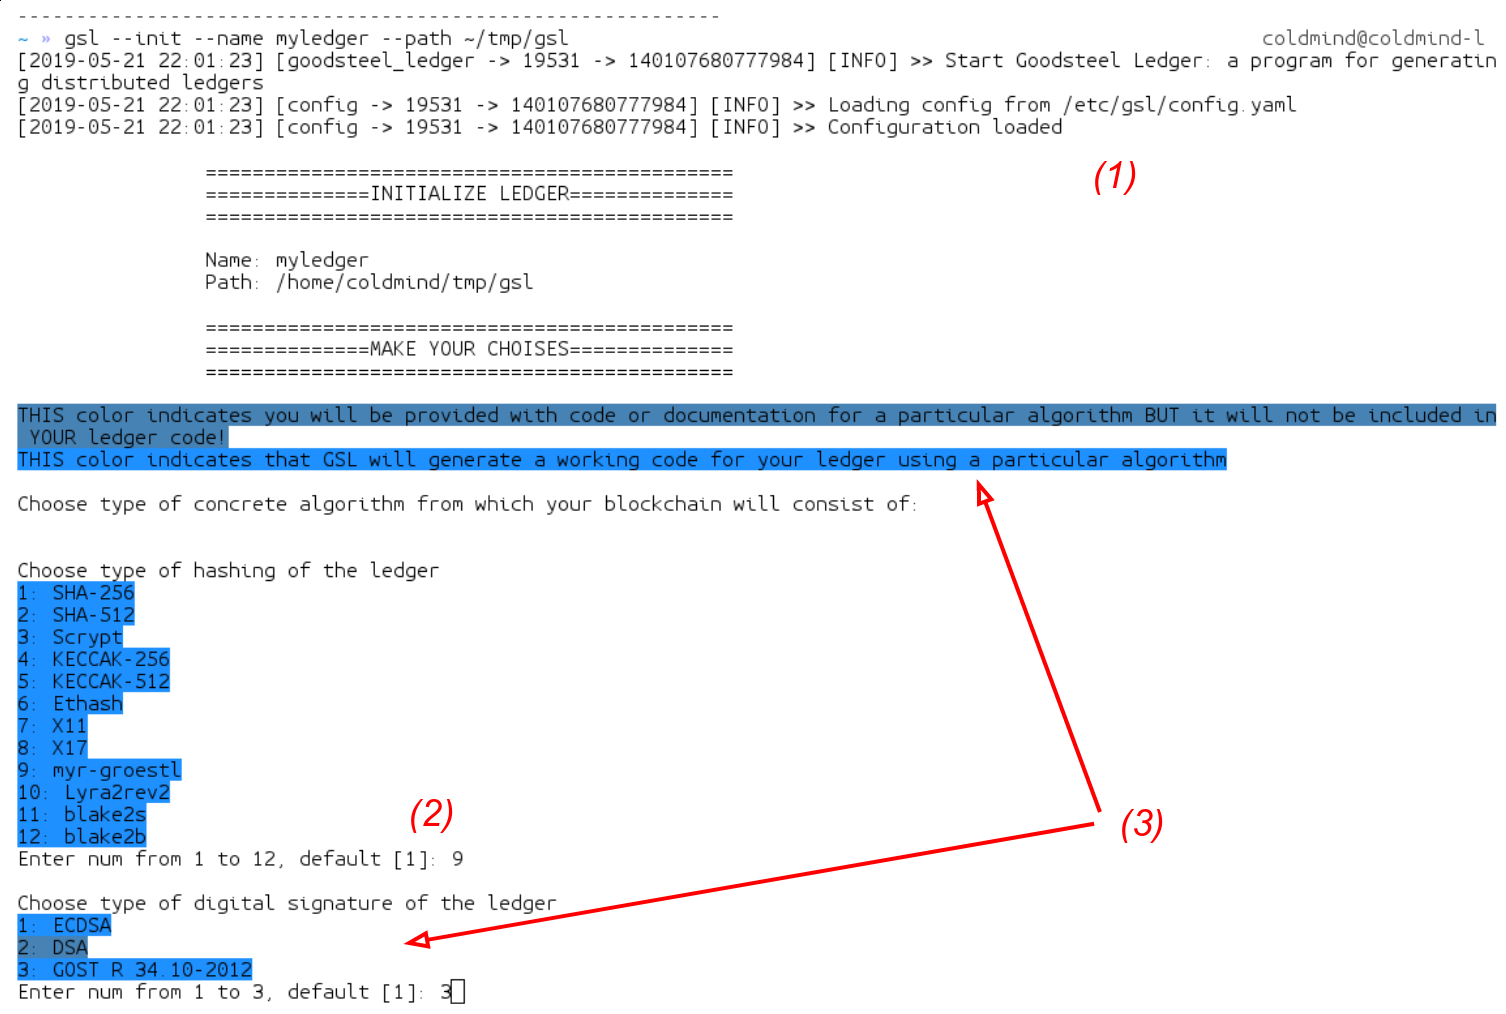
\includegraphics[width=0.85\textwidth]{./screenshots/algs_choose}
    \caption{Начало работы компоновщика}\label{algs_choose}
\end{figure}

Алгоритмы должны отображаться пронумерованно; по категориям (Рис.~\ref{algs_choose})

Вывод алгоритмов должен быть в цвете, обозночающим степень поддержки программой
алгоритма (пункт 3 Рис.~\ref{algs_choose})

Должен поддерживаться выбор алгоритмов ``по умолчанию'', и при отсутствии ввода
определённого номера алгоритма, выбираться указанный в качестве алгоритма ``по
умолчанию'' (пункт 2 Рис.~\ref{algs_choose})

\begin{figure}[h!]
    \centering
    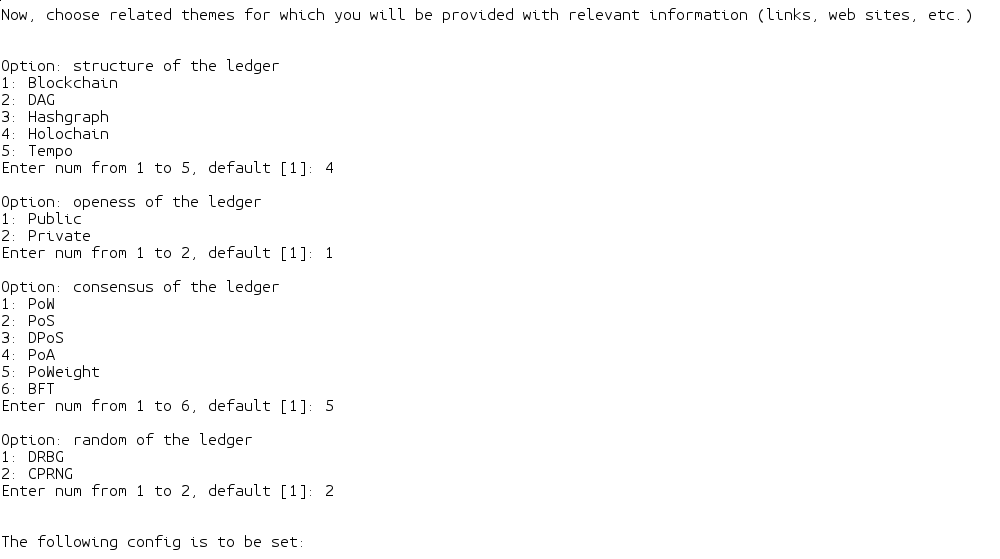
\includegraphics[width=\textwidth]{./screenshots/additional_opts}
    \caption{Вывод опций по которым будет дана справочная информация}\label{additional_opts}
\end{figure}

После выбора алгоритмов хэширования и цифровой подписи, пользователю должны
показываться свойства/структура/другие алгоритмы распределённых реестров, по
которым можно получить справочную информацию (Рис.~\ref{additional_opts})

\begin{figure}[h!]
    \centering
    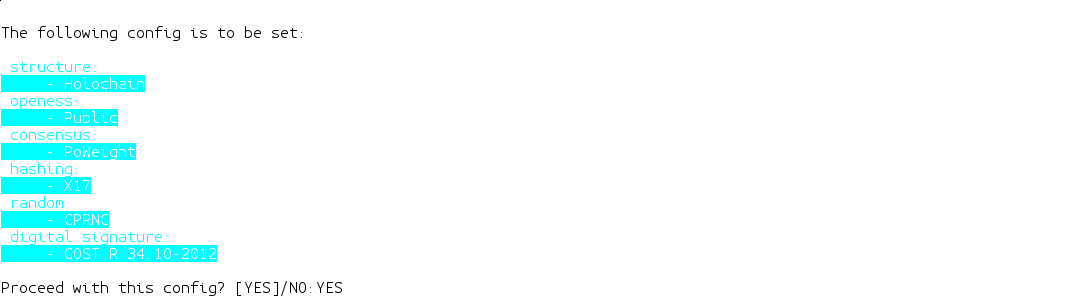
\includegraphics[width=\textwidth]{./screenshots/confirmation}
    \caption{Подтверждение выбранных опций}\label{confirmation}
\end{figure}

Должен выводиться итоговый выбор пользователя с вопросом о намерении принять
изменения и продолжить дальнейшее выполнение программы
(Рис.~\ref{confirmation})

\begin{figure}[h!]
    \centering
    \minipage{0.49\textwidth}
    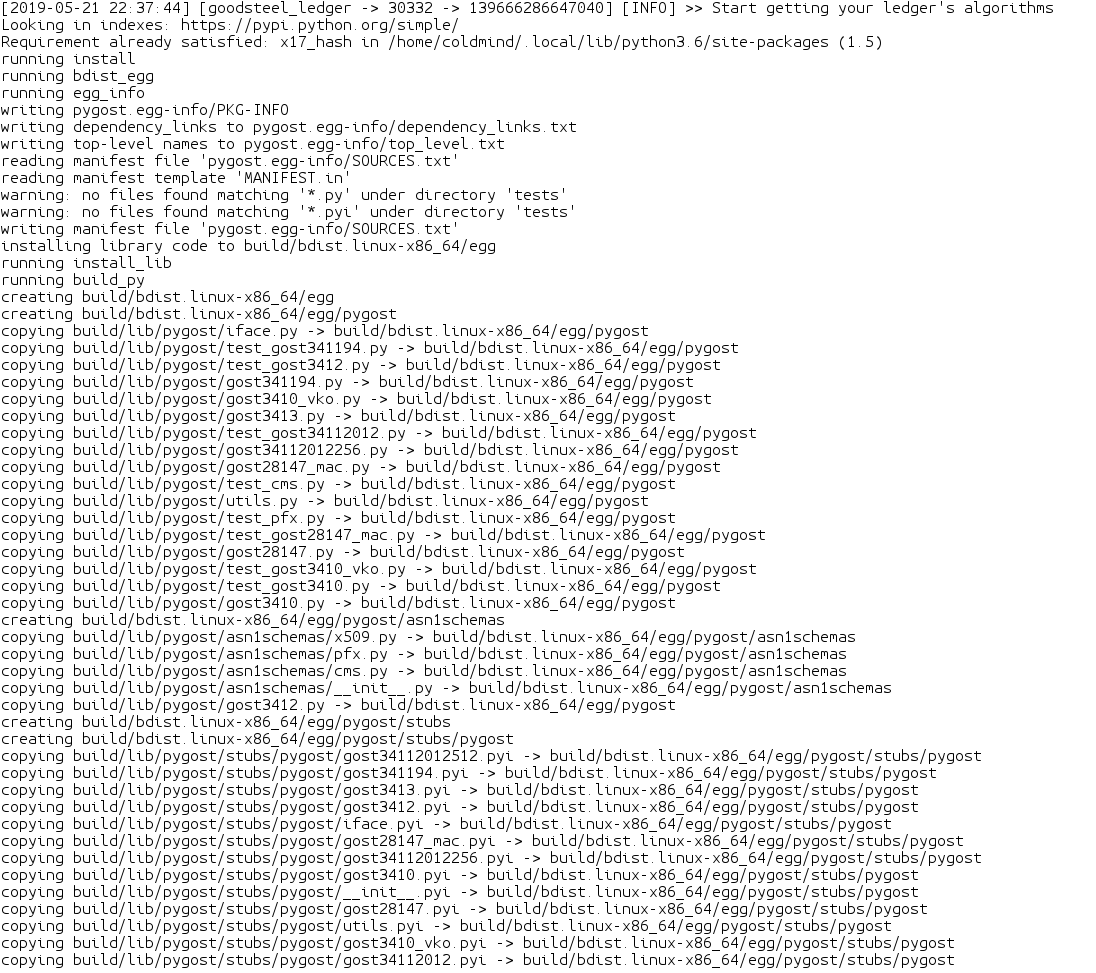
\includegraphics[width=\textwidth]{./screenshots/installing1}
    \caption{Процесс установки выбранных алгоритмов}
    \label{inst1}
    \endminipage\hfill
    \minipage{0.49\textwidth}
    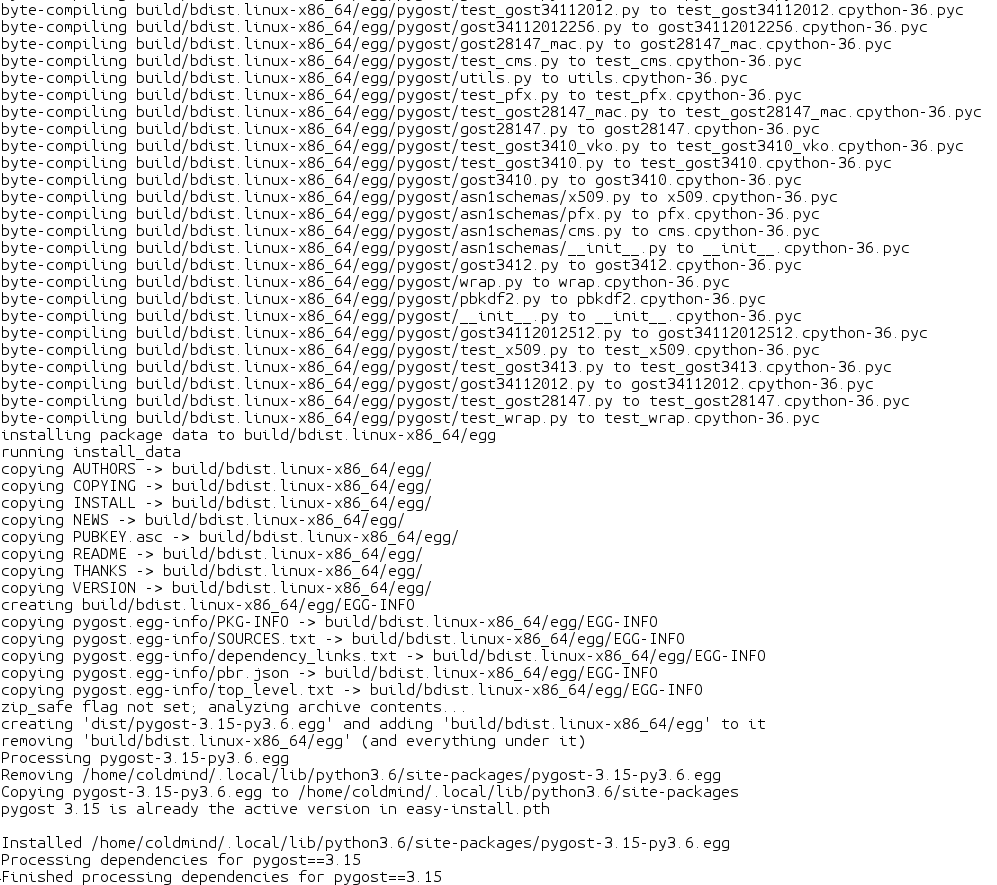
\includegraphics[width=\textwidth]{./screenshots/installing2}
    \caption{Завершение установки выбранных алгоритмов}
    \label{inst2}
    \endminipage{}
\end{figure}

При подтверждении выбора набора алгоритмов пути до исходных кодов алгоритмов
должны быть получены из хранилища, и по ним должна произойти установка в
систему (Рис.~\ref{inst1}~-~\ref{inst2}).

\begin{figure}[h!]
    \centering
    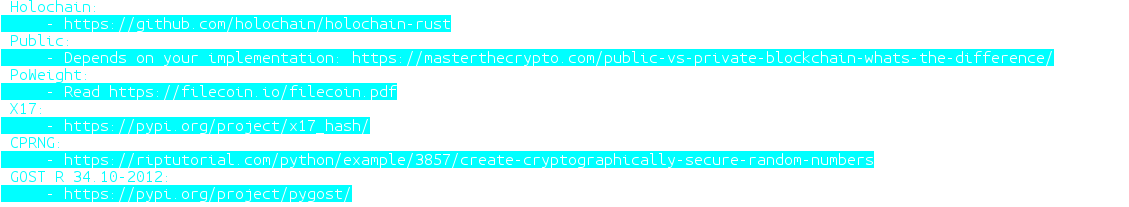
\includegraphics[width=\textwidth]{./screenshots/spravka}
    \caption{Справочная информация в конце выполнения компоновщика}\label{spravka}
\end{figure}

По завершении выполнения программа должна выводить справочную информацию по
выбранным свойствам распределённого реестра (Рис.~\ref{spravka}).

\begin{figure}[h!]
    \centering
    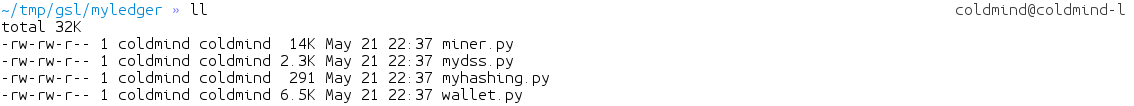
\includegraphics[width=\textwidth]{./screenshots/lldir}
    \caption{Директория со сгенерированным кодом}\label{lldir}
\end{figure}

После завершения работы программы по указанной директории должны располагаться
модули {\small wallet.py} и {\small miner.py} вместе с выбранными алгоритмами
хэщирования и электронной подписи (Рис.~\ref{lldir}).

Должно производиться автообновление алгоритмов каждый день в 21:00. Каждый день
в репозитории проекта должен быть коммит в 21:00 с обновлениями алгоритмов,
если таковые имеются.


\subsubsection{Проверка требований к реализации блокчейна}
Проверка реализованного функционала продемонстрирована на скриншотах ниже.
Модуль {\small wallet.py} будем называть \textbf{кошелёк}, а {\small miner.py}
--- \textbf{майнер}.

\begin{figure}[h!]
    \centering
    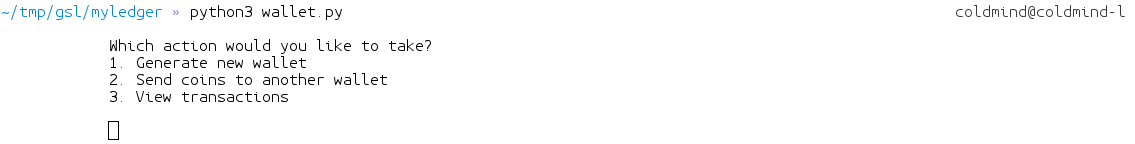
\includegraphics[width=\textwidth]{./screenshots/wallet_options}
    \caption{Возможности кошелька}\label{wallet}
\end{figure}

Возможности кошелька должны включать в себя 3 функции: генерирования нового
адреса (пары публичный и приватный ключ), отправки средств с одного адреса на
другой, а так же просмотр блокчейна (Рис.~\ref{wallet}).

\begin{figure}[h!]
    \centering
    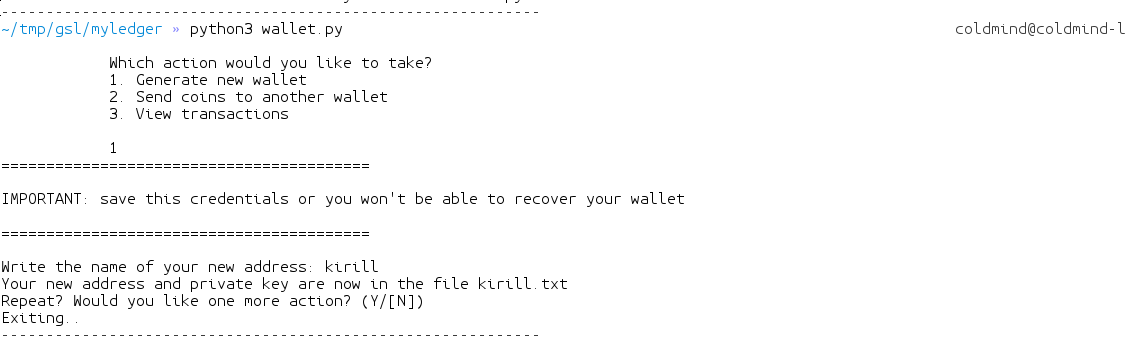
\includegraphics[width=\textwidth]{./screenshots/gen_kirill}
    \caption{Генерация адреса {\small kirill}}\label{gen_kirill}
\end{figure}

При выборе первой опции должен отображаться диалог с требованием ввести имя, и
дальнейшей генерацией адреса кошелька (пары публичный-приватный ключи) (Рис.~\ref{gen_kirill})

\begin{figure}[h!]
    \centering
    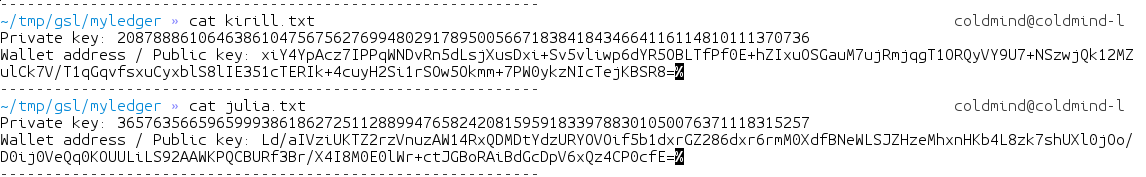
\includegraphics[width=\textwidth]{./screenshots/cat}
    \caption{Просмотр сгенерированных адресов кошельков}\label{cat}
\end{figure}

Адрес кошелька должен записываться в файл с расширением {\small .txt} и
указанным именем в названии (Рис.~\ref{cat}).

\begin{figure}[h!]
    \centering
    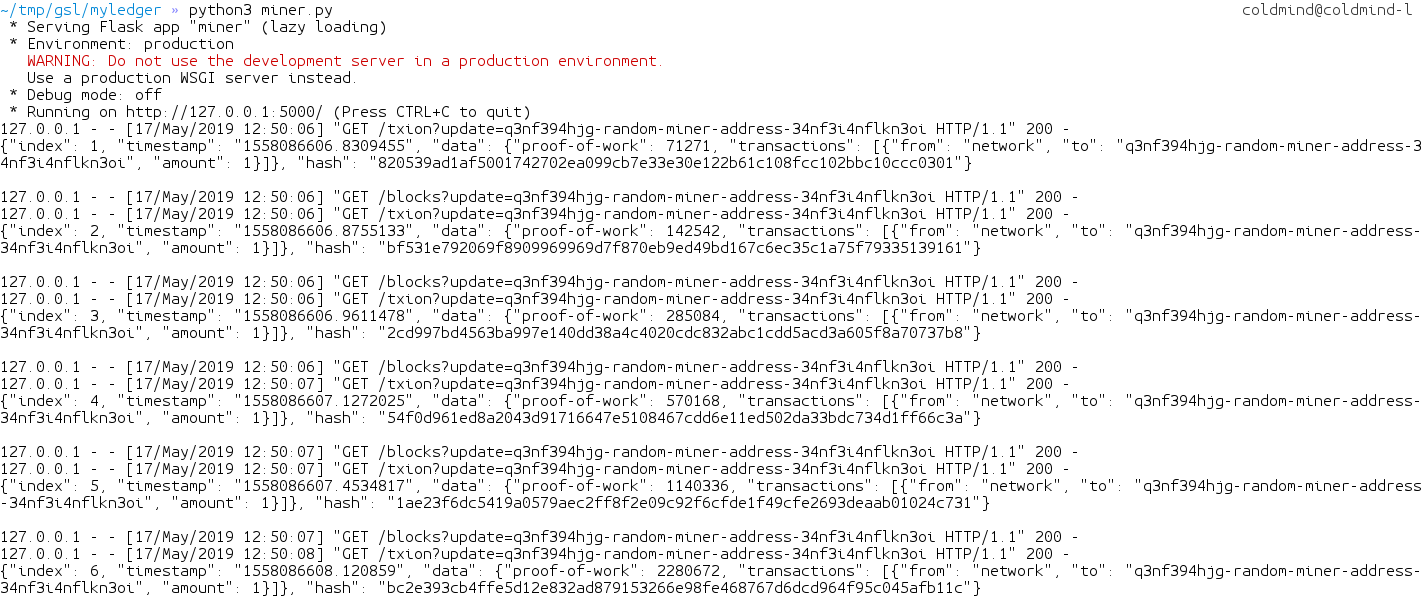
\includegraphics[width=\textwidth]{./screenshots/miner_run}
    \caption{Лог работы майрена}\label{log1}
\end{figure}

\begin{figure}[h!]
    \centering
    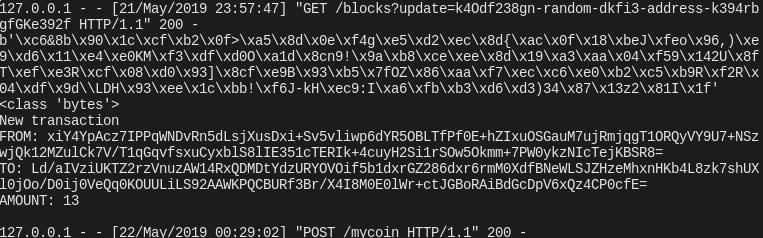
\includegraphics[width=\textwidth]{./screenshots/log_send}
    \caption{Лог регистрации новой транзакции}\label{log2}
\end{figure}

При запуске майнера, должен вестись лог о проведённых транзакциях и их
валидациях (Рис.~\ref{log1}~-~Рис.~\ref{log2}).

\begin{figure}[h!]
    \centering
    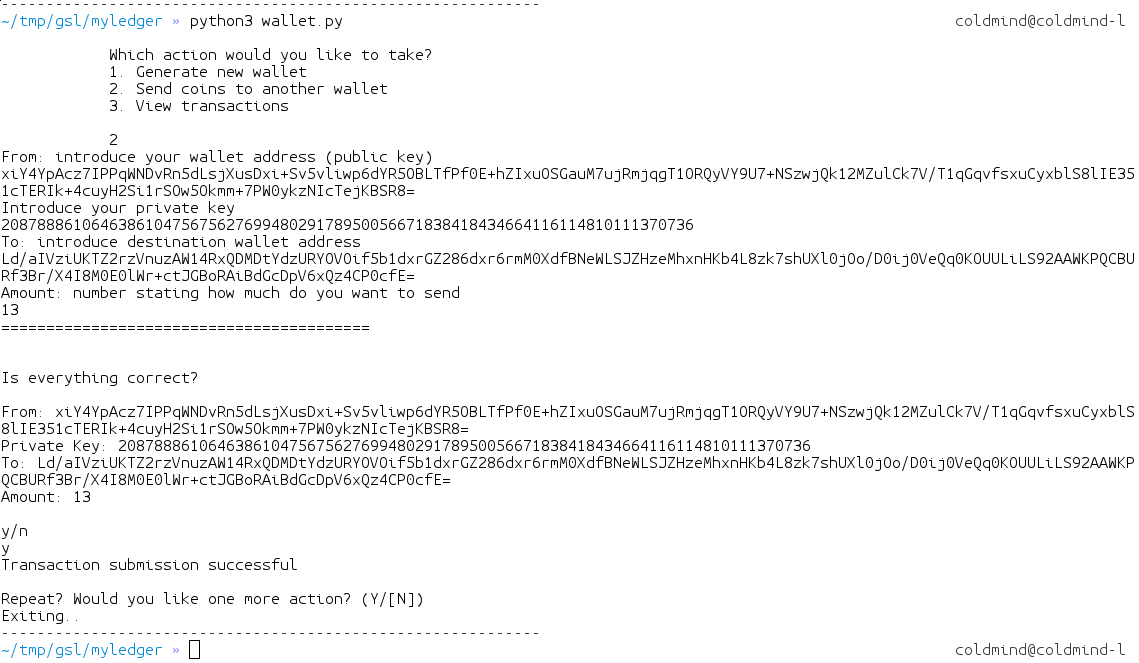
\includegraphics[width=\textwidth]{./screenshots/sending}
    \caption{Процесс отправки средств}\label{sending}
\end{figure}

В кошельке при отправке условных средств с одного счёта на другой, должны
требоваться публичный и приватный адреса отправителя, а так же публичный ключ
получателя (Рис.~\ref{sending}).

\begin{figure}[h!]
    \centering
    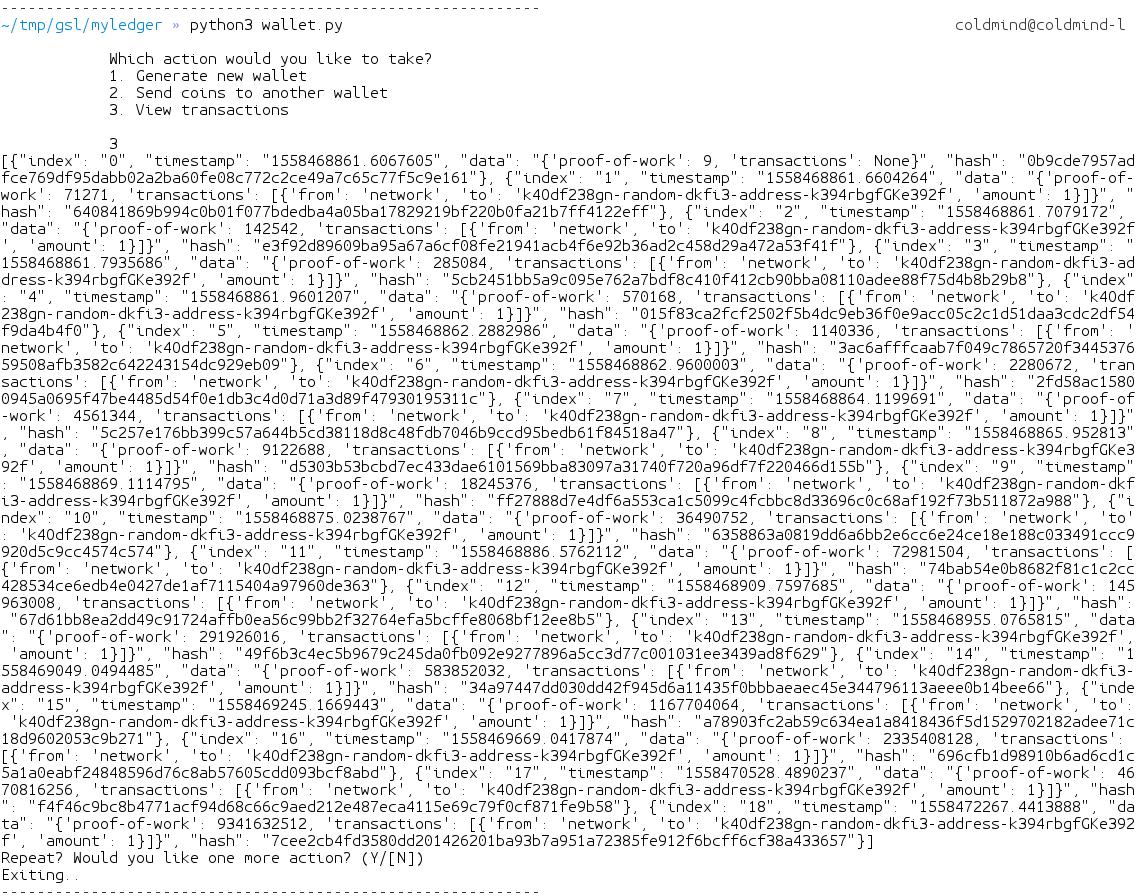
\includegraphics[width=\textwidth]{./screenshots/full_chain}
    \caption{Отображение полной цепочки транзакций}\label{full_chain}
\end{figure}
При выборе третей опции в кошельке, должен отобразиться полная цепочка
транзакций (блокчейн) (Рис.~\ref{full_chain}).

\newpage
\subsection{Проверка требований к временным характеристикам}
\subsubsection{Проверка требований к компоновщику}
Время запуска приложения не должно превышать 1.05 секунд (Рис.~\ref{launch})

\begin{figure}[h!]
    \centering
    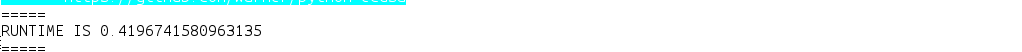
\includegraphics[width=0.7\textwidth]{./screenshots/runtime}
    \caption{Лог замера времени}
    \label{launch}
\end{figure}

Все временные требования должны быть соблюдены.
\subsubsection{Реализация блокчейна}
Временные требования к работе реализации блокчейна (майнера и кошелька) не предъявлялись.
